\chapter{Discussion}
\label{c:discussion}
\IMRADlabel{discussion}



In this chapter we analyze the results from~\autoref{c:experiments} and set them into context with results from related work. We will split all the discussion on the different environments first and then discuss the overall performance of the \algname algorithm.

\section{Model Performance}
	% TODO: Energieverlust besser als Energiezunahme ergibt Sinn, da lineare Systeme gegen Null oder Unendlich gehen (exponential decay).

	\subsection{Proof-of-Concept: LGDS}
		As we have seen in~\autoref{fig:lgdsRollout}, the \ac{lgds} proof-of-concept environment works pretty well and the true data is perfectly predicted. Applying the \ac{nrmse} to the smoothed trajectory and the rollout, the model has an error of approximately \( 0.0001 \) for every metric.

		This shows that our model is a real extension of the linear \ac{lgds} algorithm, as it is also able to produce really good results on plain linear systems.
	% end

	\subsection{Pendulum}
		The pendulum is the first environment where it gets really interesting as it is the first nonlinear environment we assess.

		As we have seen in the experiment for different latent dimensionalities, we need at least \(10\) latent dimensions to model the pendulum with a decent prediction error, where we expected some downsides on the prediction and expected a really good rollout in the training area. As we have seen in the results for a ten-dimensional latent in~\autoref{subsubsec:pendulumL10}, we see a good rollout in the training area and also a good prediction for the pendulum position, but a slightly smaller amplitude on the velocity side. This corresponds to an energy loss of the pendulum that should not happen as the pendulum is undamped.~\autoref{fig:pendulumEnergyL10} highlights this by showing the total, kinetic and potential energy of the system, where the rollout energy changes with time which should not happen. However, the potential energy almost matches the true potential energy, supporting our inspection that the position is well fit. The kinetic energy, generated by the velocity, is on the other hand a bit off. We can further inspect this behavior by looking at the rollout in the latent space in~\autoref{fig:pendulumLatentRolloutL10}. We see that the energy loss is primarily happening in the tenth dimension. Looking at the real parts of the eigenvalues of the latent state dynamics matrix,
		\begin{equation*}
			\sigma = \{ 1.00, 1.00, 1.00, 0.96, 0.65, 0.67, 0.86, 0.80, 0.73, 0.75 \}
		\end{equation*}
		we see that not all are close to one, \ac{ie} they vanish after some time. This directly corresponds to the energy loss in the system (the eigenvalues of a system capture the time evolution). We also see that the tenth dimension has a really high variance in its states, indicating that the model is unsure what to do with that dimension. Looking at the rollout of a nine-dimensional latent in~\autoref{fig:pendulumRolloutL09}, however, we see that the energy loss is still there. It also does not make sense to inspect higher-dimensional latent spaces for now as we have seen in the latent dimensionalities experiment that the error does not shrink much and the 14-dimensional latent that we inspected in~\autoref{subsubsec:pendulumL10} does also loose energy. We do not expected this to get better with higher latent dimensionalities. Also, higher dimensionalities impose numerical instability, a phenomenon we will address in~\autoref{subsec:discussPerformanceNumerics}.

		For this environment, we get really small confidences with the true trajectory still lying in the region of confidence. We also see that the variance is higher on the turns of the pendulum which makes sense as that is the most critical part of the movement.

		While these first results cast a shadow on our model performance, the energy loss builds hope for the damped pendulum to work out well.

		\begin{figure}
			\centering
			\begin{subfigure}{0.7\linewidth}
				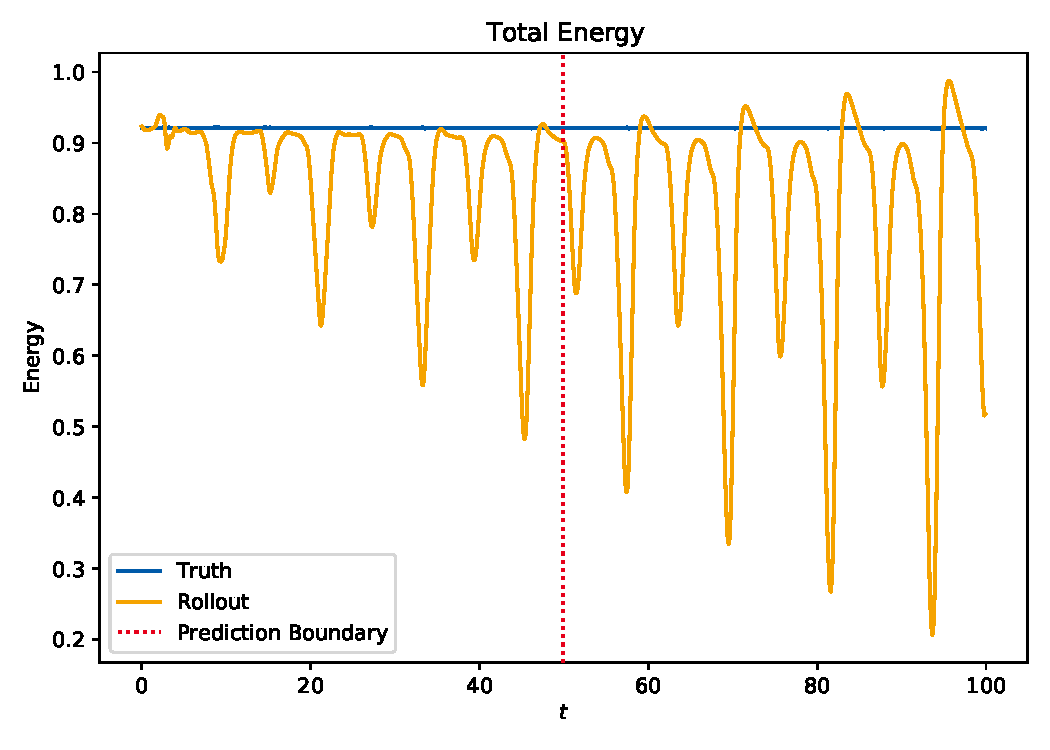
\includegraphics[width=\linewidth]{figures/results/pendulum/run-latent-dim-10/energy-R10-N0-total.pdf}
			\end{subfigure} \\
			\begin{subfigure}{0.5\linewidth}
				\centering
				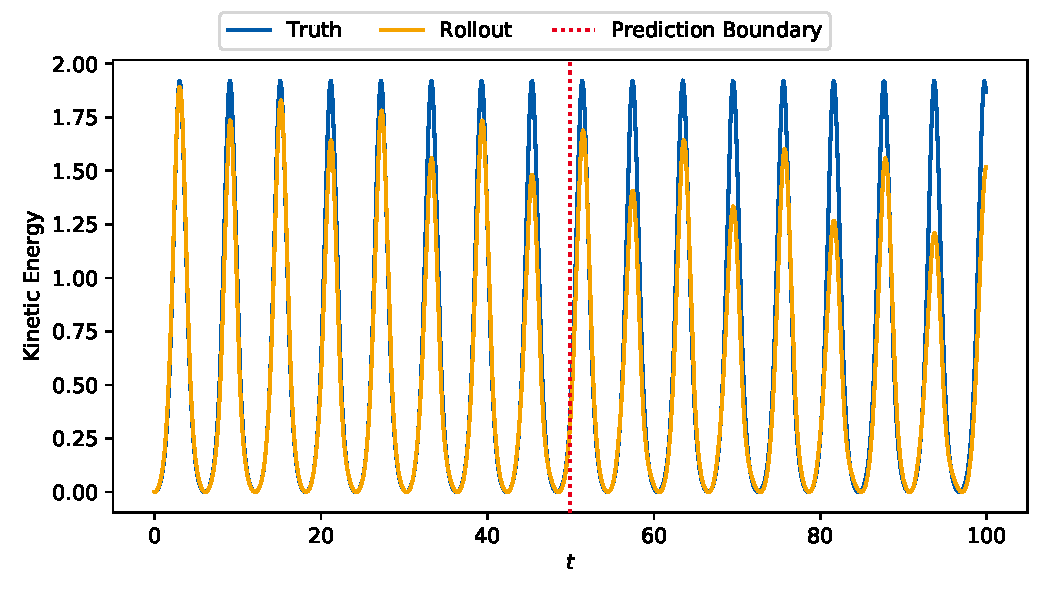
\includegraphics[width=\linewidth]{figures/results/pendulum/run-latent-dim-10/energy-R10-N0-kinetic.pdf}
			\end{subfigure}%
			~
			\begin{subfigure}{0.5\linewidth}
				\centering
				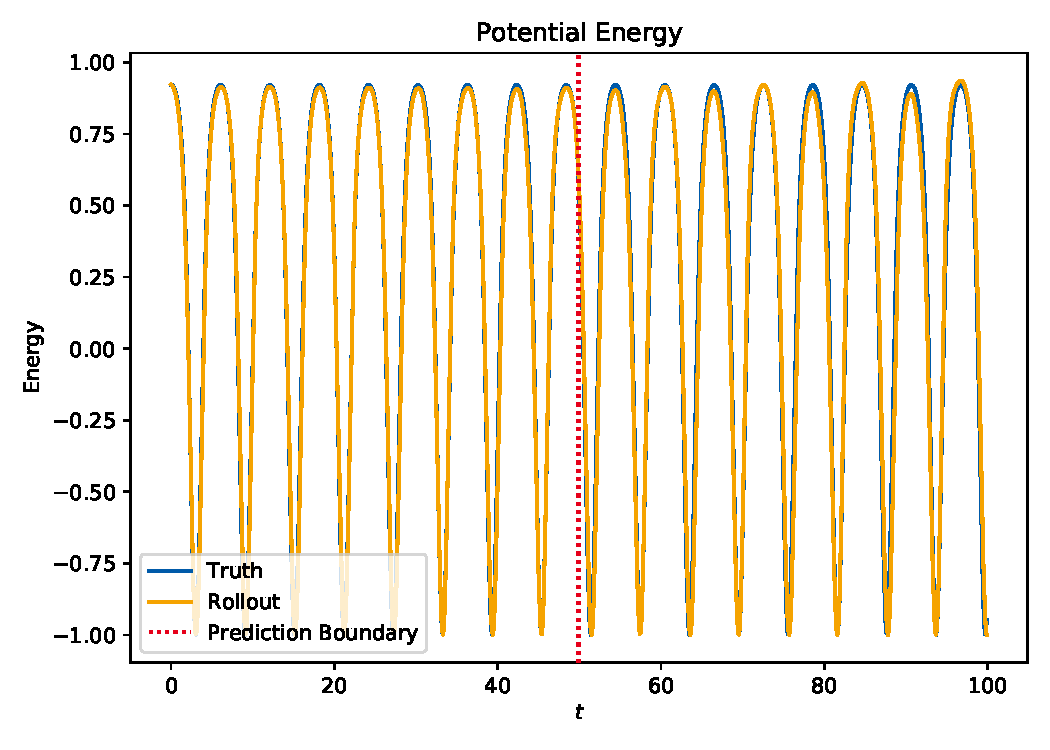
\includegraphics[width=\linewidth]{figures/results/pendulum/run-latent-dim-10/energy-R10-N0-potential.pdf}
			\end{subfigure}
			\caption{Total energy of the undamped pendulum composed of the kinetic energy on the bottom left and the potential energy on the bottom right. The blue line represents the true energy, calculated from the training and validation data. The orange line is the energy calculated from the rollout. As usual, the red line is the prediction boundary until all training data was used and the rest is prediction.}
			\label{fig:pendulumEnergyL10}
		\end{figure}

		\begin{figure}
			\centering
			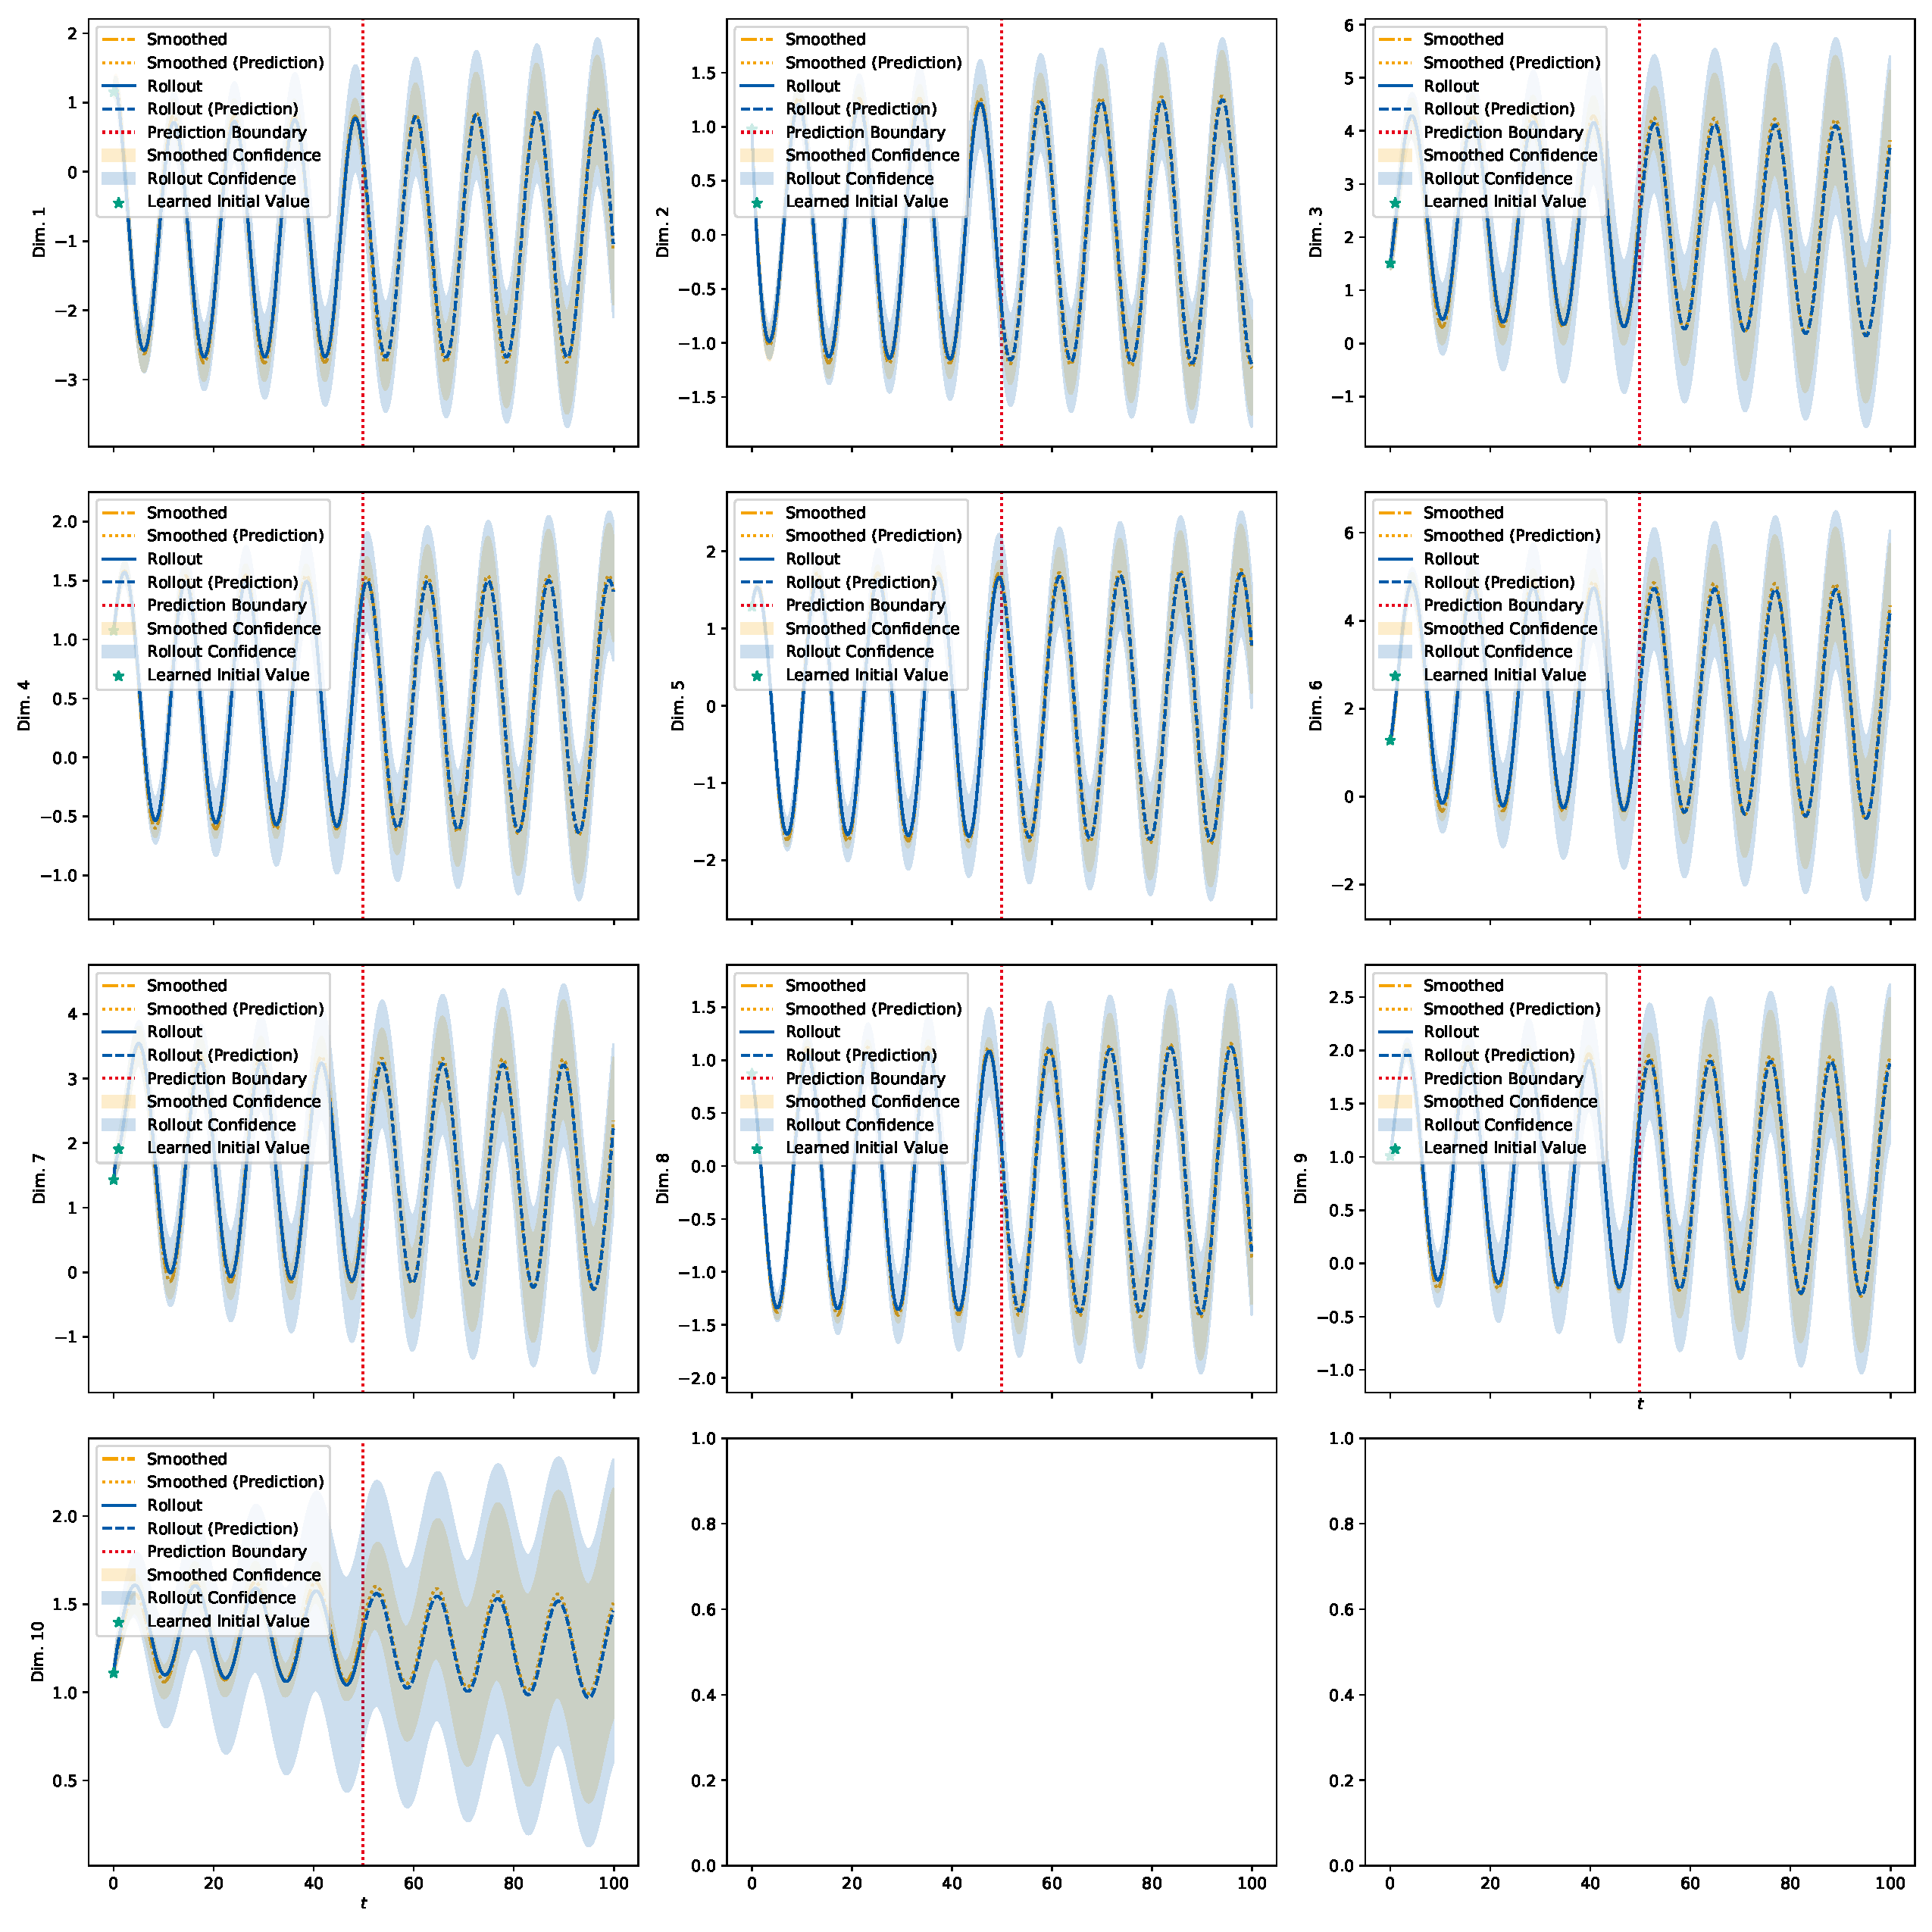
\includegraphics[width=\linewidth]{figures/results/pendulum/run-latent-dim-10/rollout-latents-N0.pdf}
			\caption{Rollout of the latent dimensions of the pendulum environment for \(k = 10 \) latents.}
			\label{fig:pendulumLatentRolloutL10}
		\end{figure}

		\begin{figure}
			\centering
			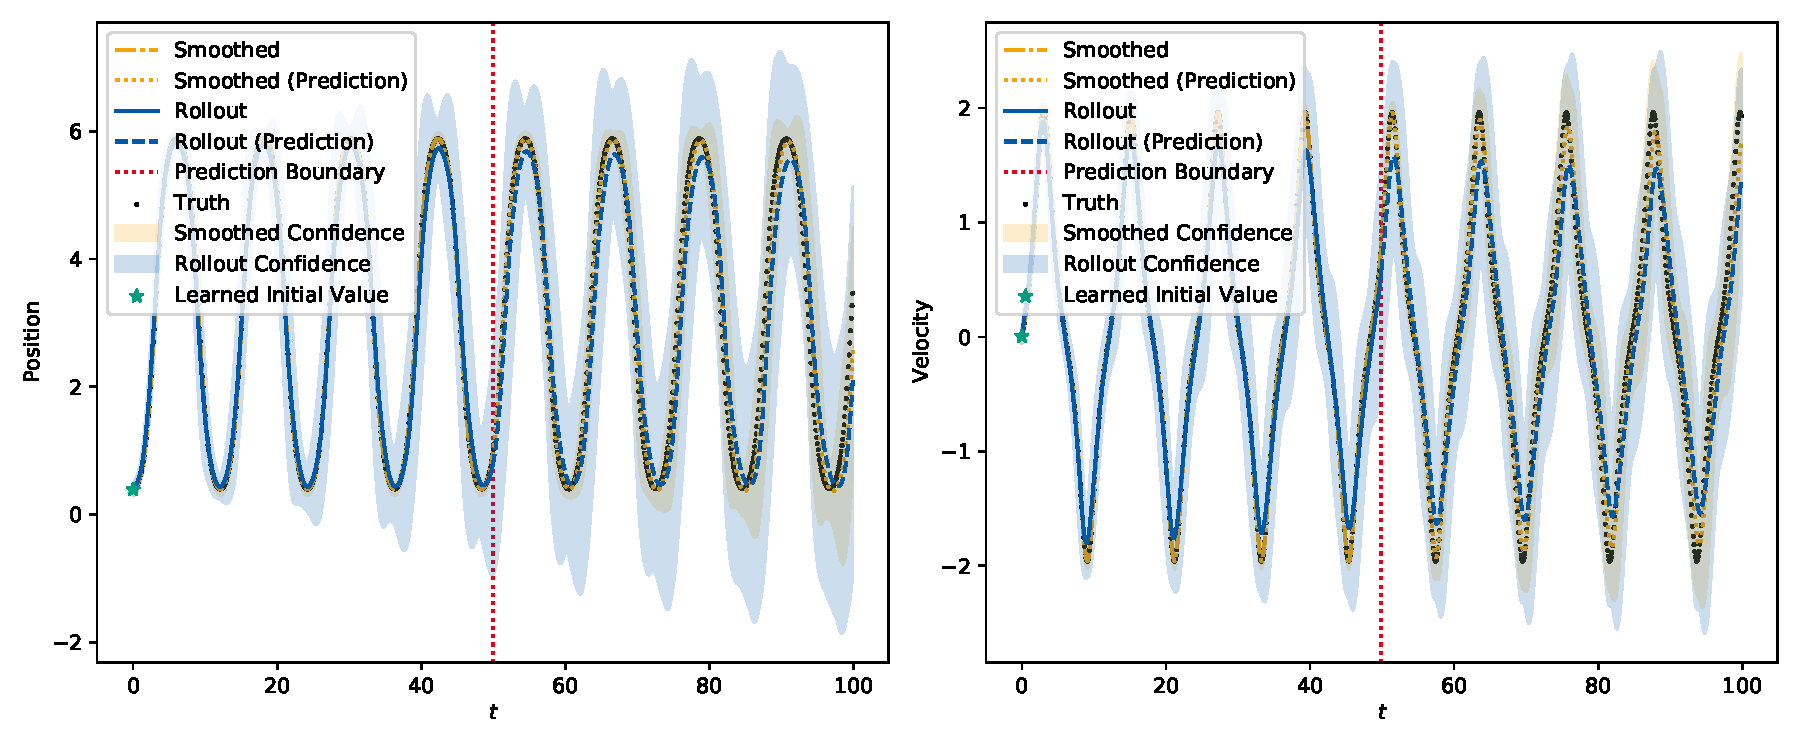
\includegraphics[width=\linewidth]{figures/results/pendulum/run-latent-dim-09/rollout-observations-N0.pdf}
			\caption{The rollout plot in the observation space of the pendulum environment for \(k = 9\). The left plot shows the displacement and the right plot the angular velocity. The black dots represent the true data of which the model used everything till the red prediction boundary to train on. The blue line is the rollout, starting from the learned initial value (marked with a green star). The orange dash-dotted line is the smoothed data. The dotted orange line then is the rollout starting from the last smoothed state, forming the "smoothed prediction". The shaded regions show the confidence, \ac{ie} two times the standard deviation.}
			\label{fig:pendulumRolloutL09}
		\end{figure}
	% end

	\subsection{Damped Pendulum}
		As for the undamped pendulum, we have seen in the experiment with different latent dimensionalities that we need at least ten latent dimensions. For ten dimensions, we get a decent \ac{nrmse} on both training and prediction. We have seen this behavior in~\autoref{subsubsec:pendulumDampedL10} and in the rollout plot in~\autoref{fig:pendulumDampedRolloutL10}. In contrast to the undamped pendulum, the amplitudes of the oscillations are now on the correct heights, so we definitely learn the energy loss of the system. We can also see this behavior in the plot of the total, kinetic and potential energy in~\autoref{fig:pendulumDampedEnergyL10}. We see in the total and the kinetic and potential energy that the damped pendulum model is really close to the real energy levels, in all energy types. This supports the first interpretation of the rollout that we really learn the energy loss. On the other hand, the rollout is phase-shifted to the real trajectory, sometimes even predicting the pendulum to be on the opposite side of a swing. Looking at the rollout in the latent space in~\autoref{fig:pendulumDampedLatentRolloutL10}, we see a similar behavior in the latent space, so our learned observation function seems to be correct, but the latent dynamics are a bit off.

		Improving this might be possible by fixing the observation function and optimizing just the state dynamics matrix on its own. This reduces the parameters the algorithm has to learn by a lot, possibly yielding a more accurate rollout. But overall we are happy with this result as we learn the energy loss and get a confidence that is not too high such that the real position is still in the region of variance. As for the undamped pendulum, we get higher variances in regions where the pendulum turns over.

		\begin{figure}
			\centering
			\begin{subfigure}{0.7\linewidth}
				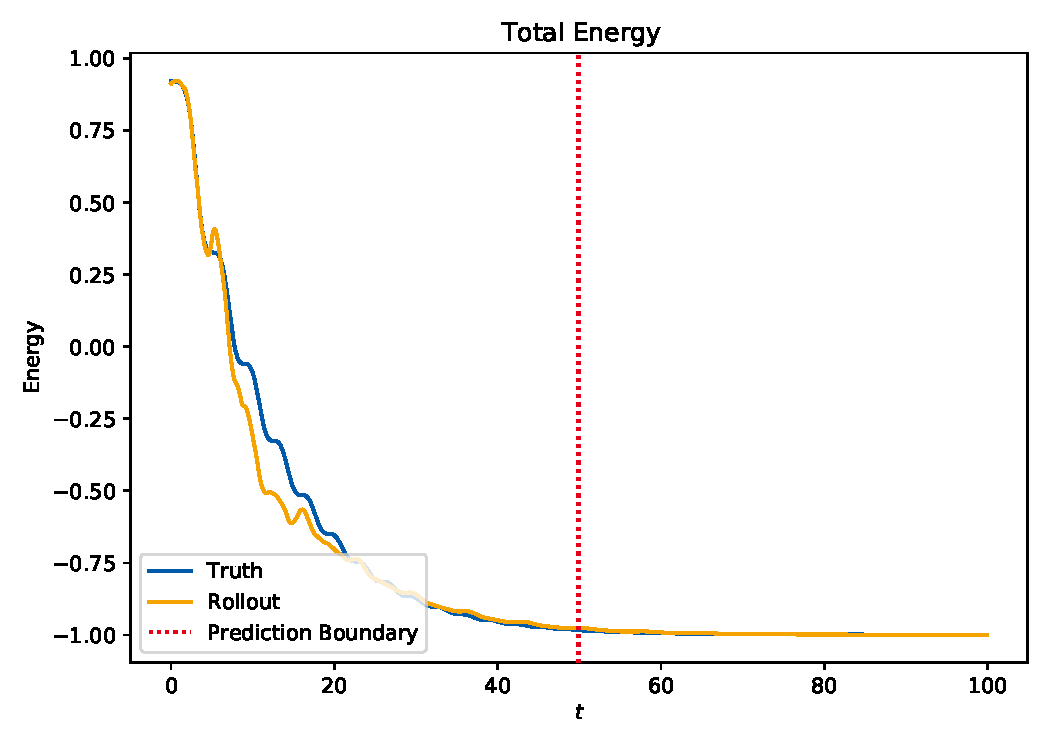
\includegraphics[width=\linewidth]{figures/results/pendulum-damped/run-latent-dim-10/energy-R110-N0-total.pdf}
			\end{subfigure} \\
			\begin{subfigure}{0.5\linewidth}
				\centering
				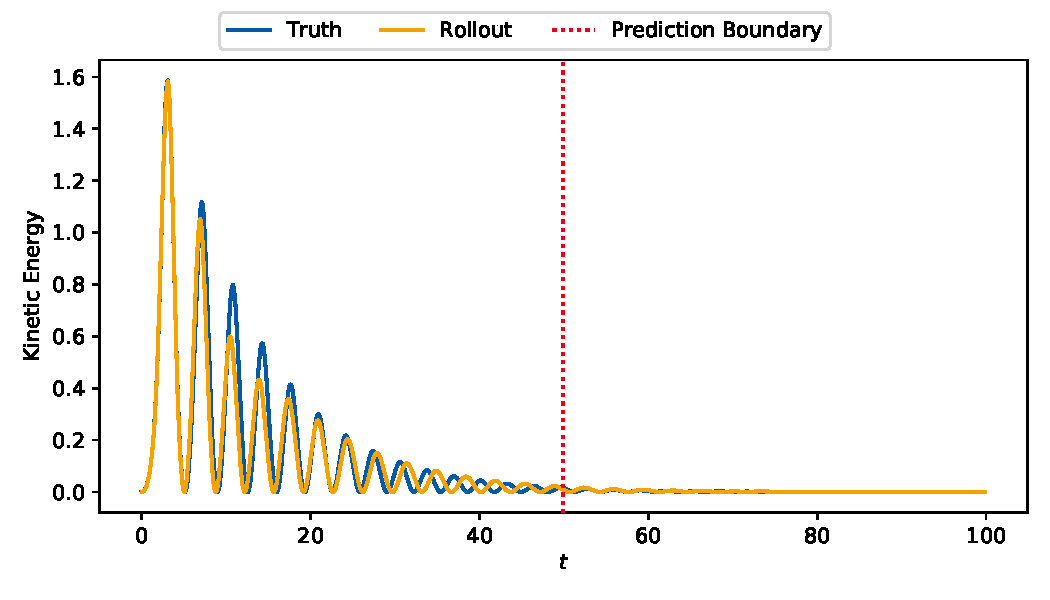
\includegraphics[width=\linewidth]{figures/results/pendulum-damped/run-latent-dim-10/energy-R110-N0-kinetic.pdf}
			\end{subfigure}%
			~
			\begin{subfigure}{0.5\linewidth}
				\centering
				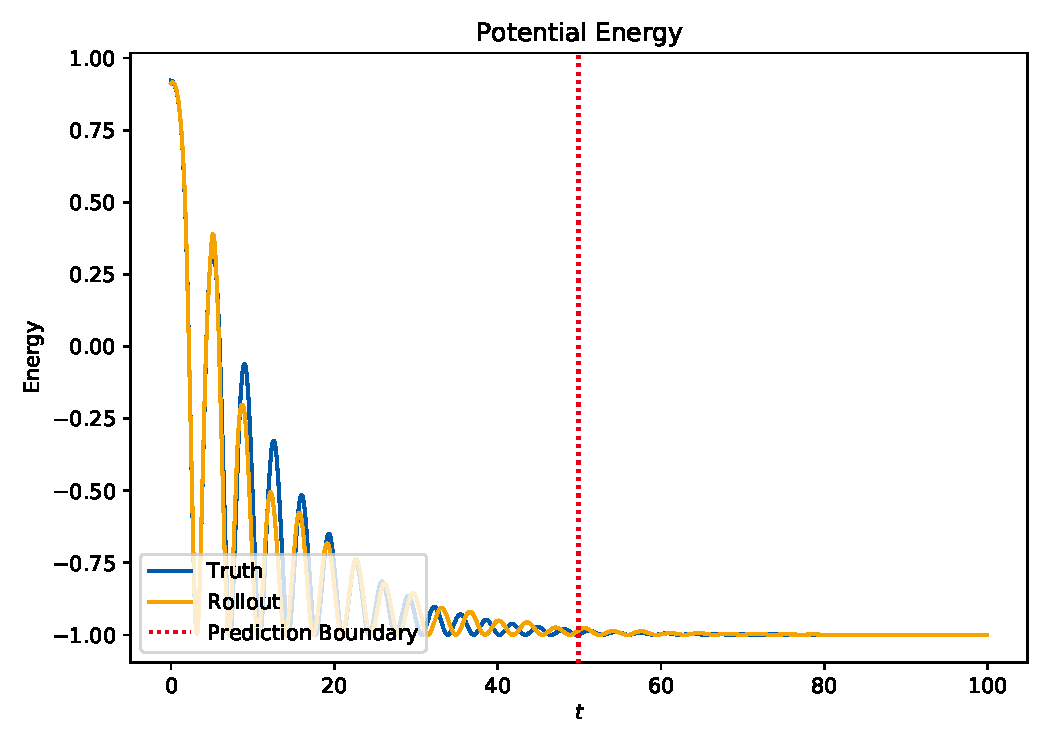
\includegraphics[width=\linewidth]{figures/results/pendulum-damped/run-latent-dim-10/energy-R110-N0-potential.pdf}
			\end{subfigure}
			\caption{Total energy of the pendulum composed of the kinetic energy on the bottom left and the potential energy on the bottom right. The blue line represents the true energy, calculated from the training and validation data. The orange line is the energy calculated from the rollout. As usual, the red line is the prediction boundary until all training data was used and the rest is prediction.}
			\label{fig:pendulumDampedEnergyL10}
		\end{figure}

		\begin{figure}
			\centering
			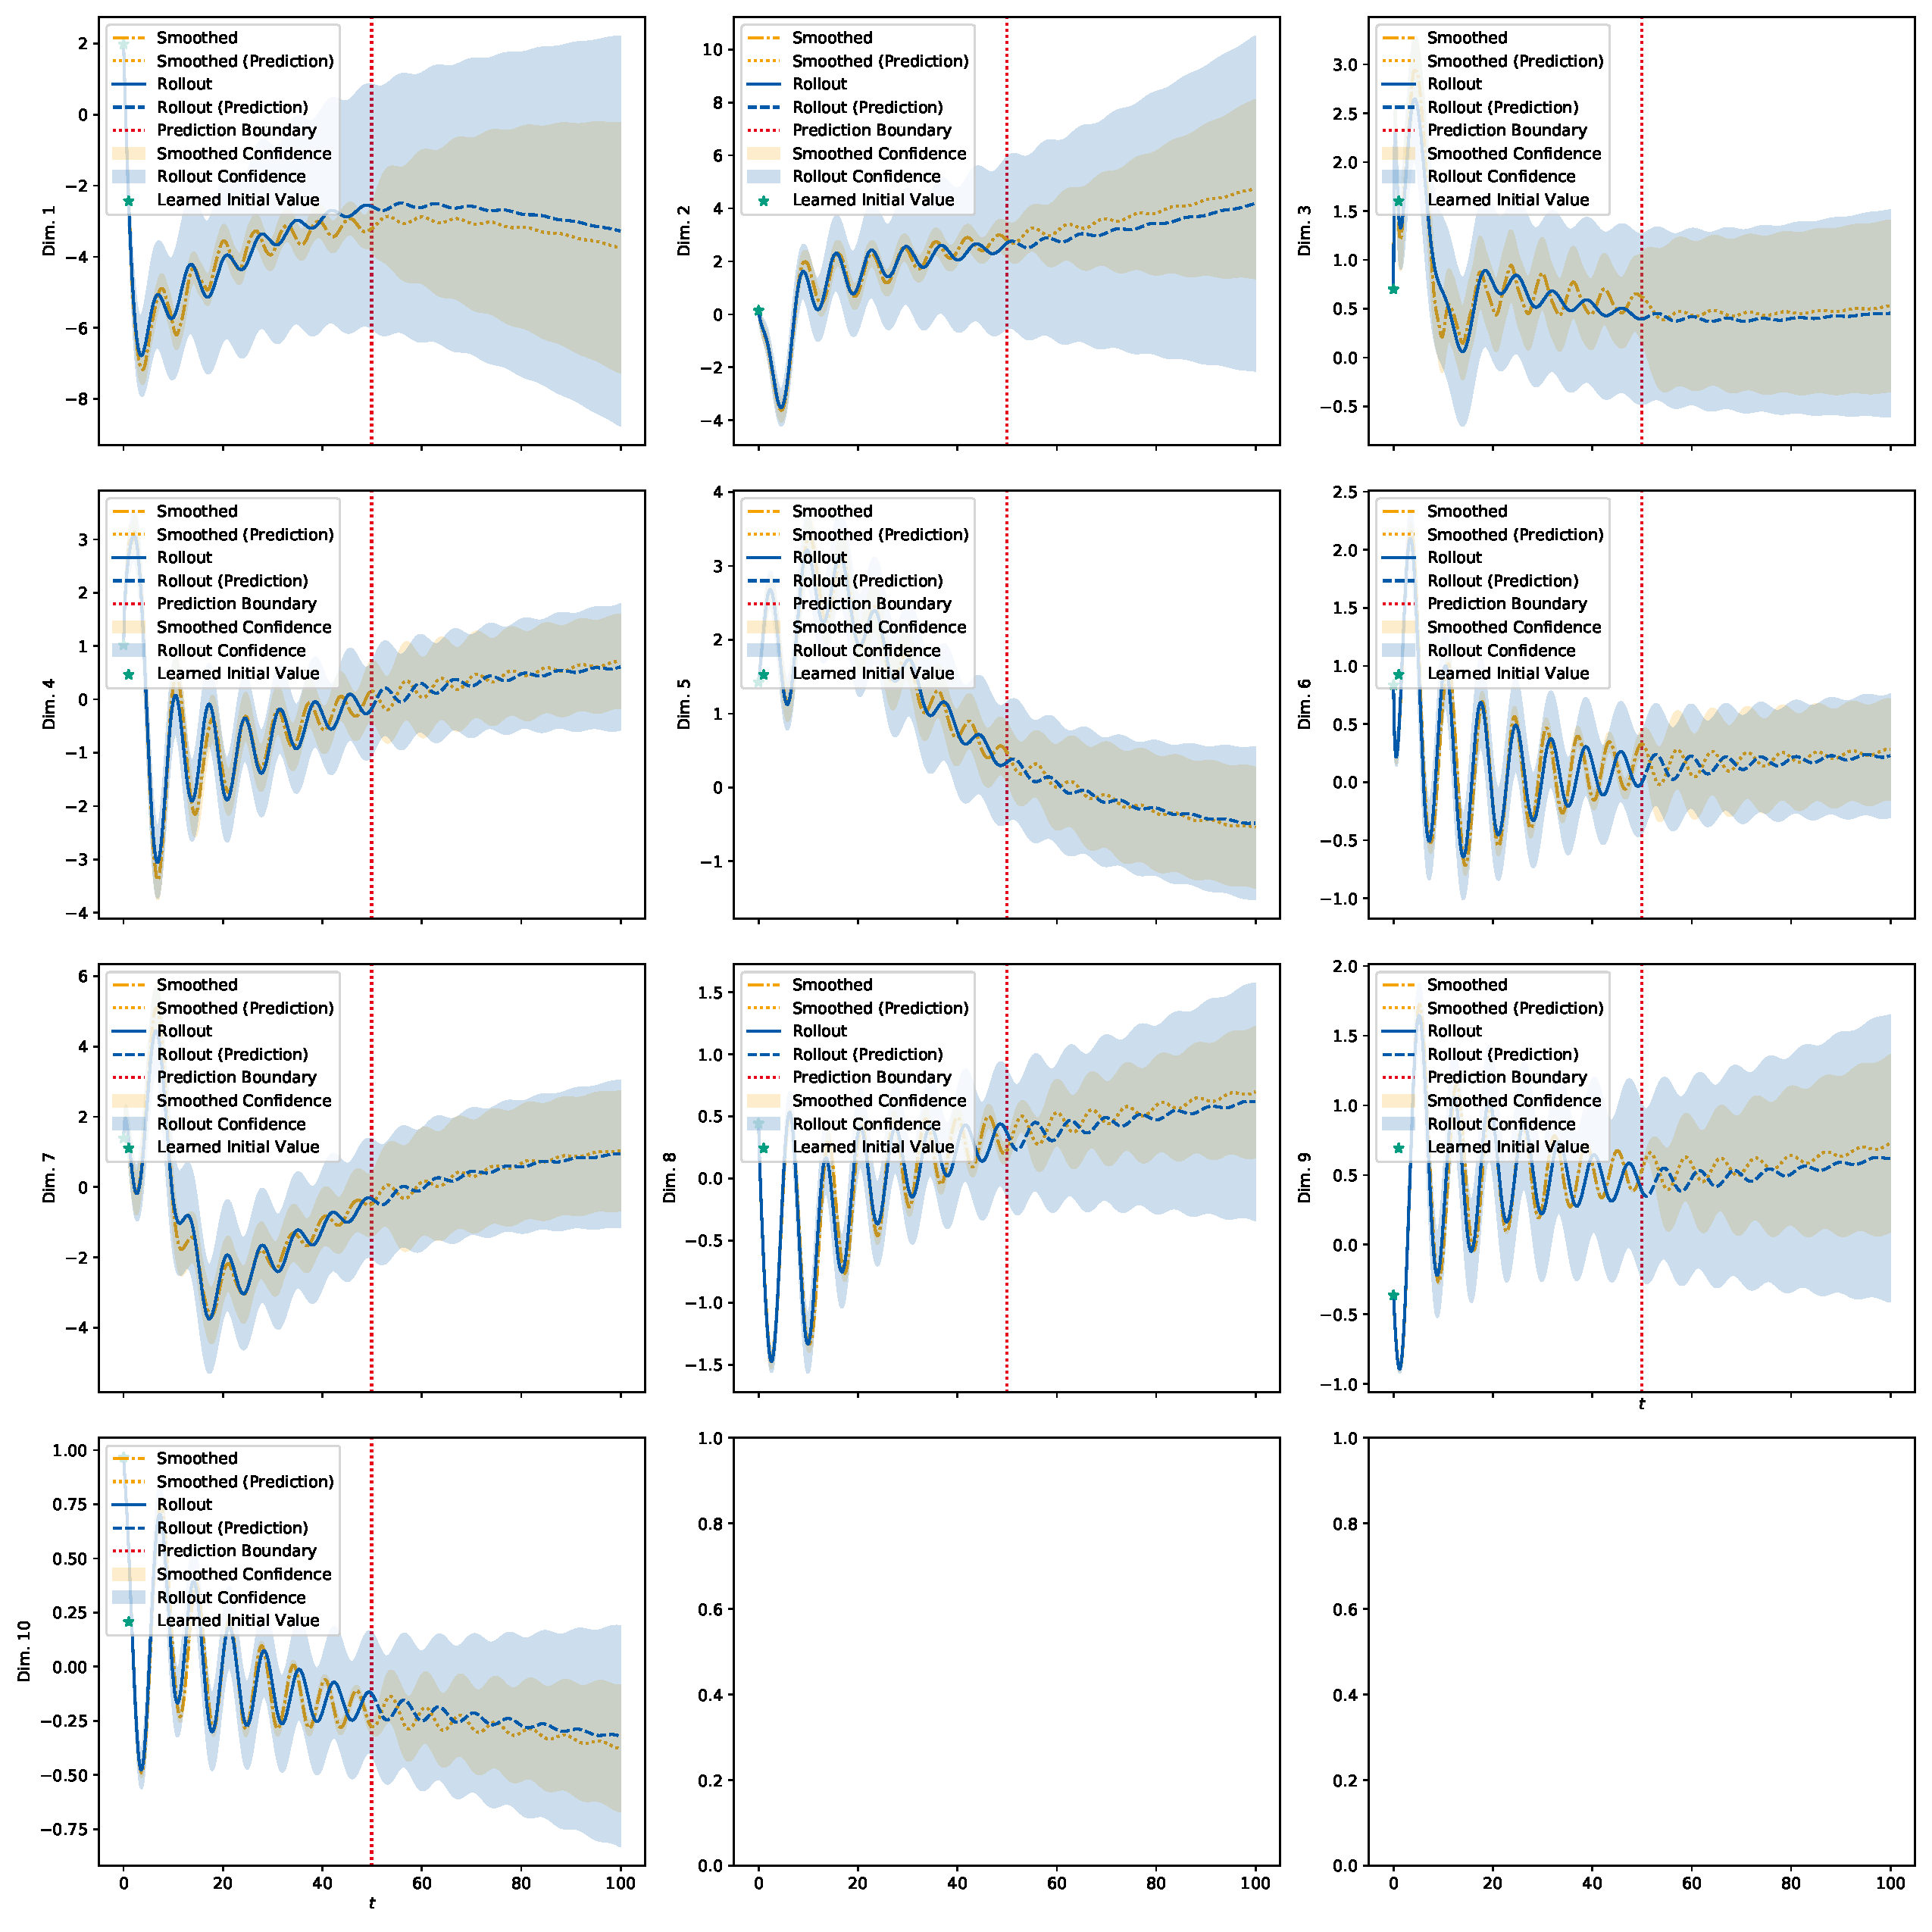
\includegraphics[width=\linewidth]{figures/results/pendulum-damped/run-latent-dim-10/rollout-latents-N0.pdf}
			\caption{Rollout of the latent dimensions of the damped pendulum environment for \(k = 10 \) latents.}
			\label{fig:pendulumDampedLatentRolloutL10}
		\end{figure}
	% end

	\subsection{Gym Pendulum}
		% TODO
	% end

	\subsection{Gym Cartpole}
		% TODO
	% end

	\subsection{Gym Double Pendulum}
		% TODO
	% end

	\subsection{Summary and Numerical Stability}
		\label{subsec:discussPerformanceNumerics}

		% TODO
	% end
% end

\section{Comparison with Related Work}
	% In-Depth Comparison with Lush et al.
	% In-Depth Comparsion with Morton et al.
	% Probably more qualitative comparisons with Sequential VAE or DVBF (Karl et al.).

	\todo{Exp: Comparison}
% end
